\documentclass[serif,xcolor=pdftex,dvipsnames,table,hyperref={bookmarks=false,breaklinks}]{beamer}

%%%%%%%%%%%%%%%%
% Change the macros below to configure the title slides
% for your course.
\newcommand{\coursename}{COMPSCI 589}
\newcommand{\instructor}{Benjamin M. Marlin}
\newcommand{\university}{University of Massachusetts Amherst}
\newcommand{\department}{College of Information and Computer Sciences}
%%%%%%%%%%%%%%%%


\newcommand{\settitlecard}[2]{
  \title[\coursename  Lecture #1] 
    {\coursename \\ Lecture #1: #2}
     \author[\instructor]{\instructor}
     \institute[\university]{
     \department\\
     \university
   }
\date{}
}

\newcommand{\maketitlepage}{
  \begin{frame}
  \titlepage
  \center{
    %If you use the slides unmodified, retain the attribution below
    \tiny{Slides by Benjamin M. Marlin (marlin@cs.umass.edu). \\
    \vspace{-1em}Created with support from National Science Foundation Award\# IIS-1350522. 
    %If you modify the slides, please retain the alternate attribution below
    %\tiny{Based on slides by Benjamin M. Marlin (marlin@cs.umass.edu). \\    
    %\vspace{-1em}Created with support from National Science Foundation Award\# IIS-1350522. 
    }                                              
  }  
  \end{frame}
}

\AtBeginSection[]
{
  \begin{frame}<beamer>{Outline}
    \tableofcontents[currentsection,subsectionstyle=hide]
  \end{frame}
}


\newcommand{\cut}[1]{}

\newcommand{\iconbox}[4]{
  \only<#1-#2>{
    \begin{columns}[T]
      \column{0.5in}
           \includegraphics[width=0.5in]{#3}
       \column{3.7in}
            #4
    \end{columns}
    \medskip
    \medskip
    \medskip
  }
}

\mode<presentation>{
  \usepackage{../beamertheme589theme}
  \setbeamercovered{invisible}
}

\mode<handout>{
  \usepackage{../beamertheme589theme}
  \setbeamercovered{transparent}
}


\usepackage[english]{babel}
\usepackage[latin1]{inputenc}
\usepackage{times}
\usepackage[T1]{fontenc}
\usepackage{amsmath}
\usepackage{amssymb}
\usepackage[noend]{algorithmic}
\usepackage{algorithm}
\usepackage{listings}

\renewcommand\mathfamilydefault{\rmdefault}

\newcommand{\setA}{\mathcal{A}}
\newcommand{\setB}{\mathcal{B}}
\newcommand{\setS}{\mathcal{S}}
\newcommand{\setV}{\mathcal{V}}
\DeclareMathOperator*{\union}{\bigcup}
\DeclareMathOperator*{\intersection}{\bigcap}
\DeclareMathOperator*{\Val}{Val}
\newcommand{\mbf}[1]{{\mathbf{#1}}}
\DeclareMathOperator*{\argmax}{arg\,max}
\DeclareMathOperator*{\argmin}{arg\,min}
\DeclareMathOperator*{\sign}{sign}
\newcommand{\deriv}[2]{\frac{\partial{#1}}{\partial{#2}}}


\settitlecard{8}{Linear Regression, Ridge, and Lasso}

\begin{document}

\maketitlepage

\section{Regression}
\subsection{Foo}

\begin{frame}[t]{Views on Machine Learning}

\iconbox{1}{}{../Figures/mitchell.jpg}{\textbf{Mitchell (1997):} ``A computer program is said to learn from experience E with respect to some class of tasks T and performance measure P, if its performance at tasks in T, as measured by P, improves with experience E.''\\[12pt]  Substitute ``training data D'' for  ``experience E.''}

\end{frame}

\begin{frame}[t]{The Regression Task}

\begin{block}{Definition: The Regression Task}
Given a feature vector $\mbf{x}\in\mathbb{R}^D$, predict it's corresponding output value $y\in \mathbb{R}$.
\end{block}

\pause
\center
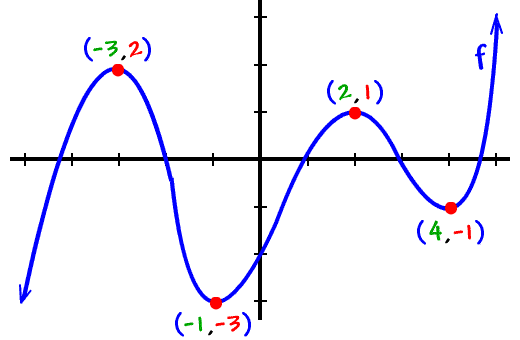
\includegraphics[width=3in]{../Figures/polynomial-function.png}
\end{frame}

\begin{frame}[t]{Example: Stock Prices}
\center
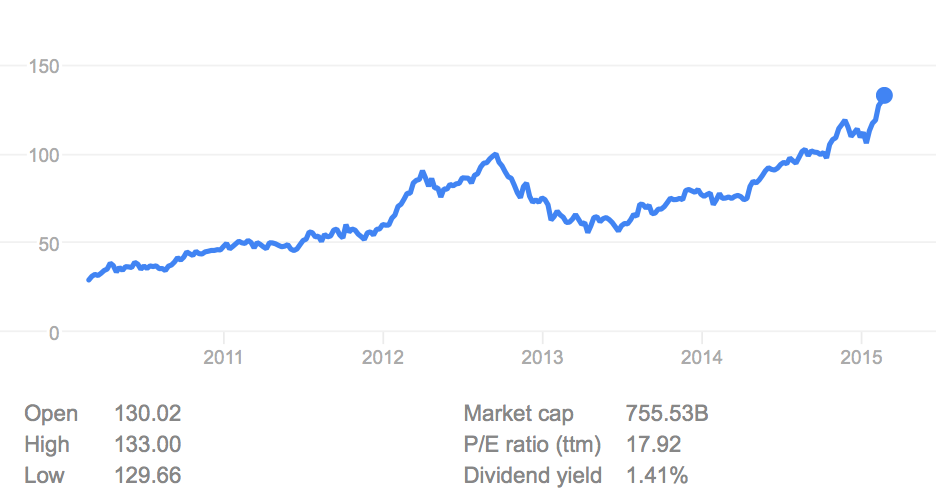
\includegraphics[width=4in]{../Figures/apple-stock.png}
\end{frame}

\begin{frame}[t]{Example: Climate Change}
\center
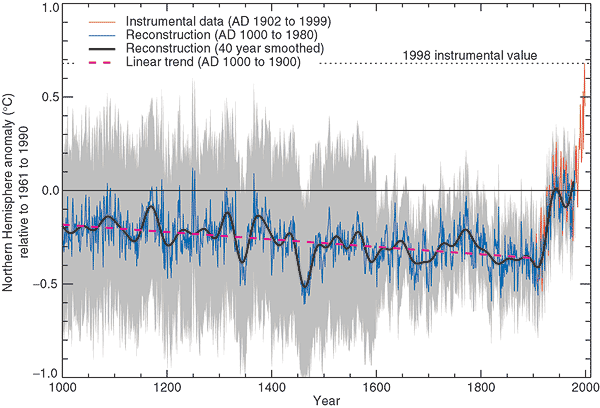
\includegraphics[width=4in]{../Figures/northern-hemisphere-temperature.png}
\end{frame}

\begin{frame}[t]{Example: Weather Forecasting}
\center
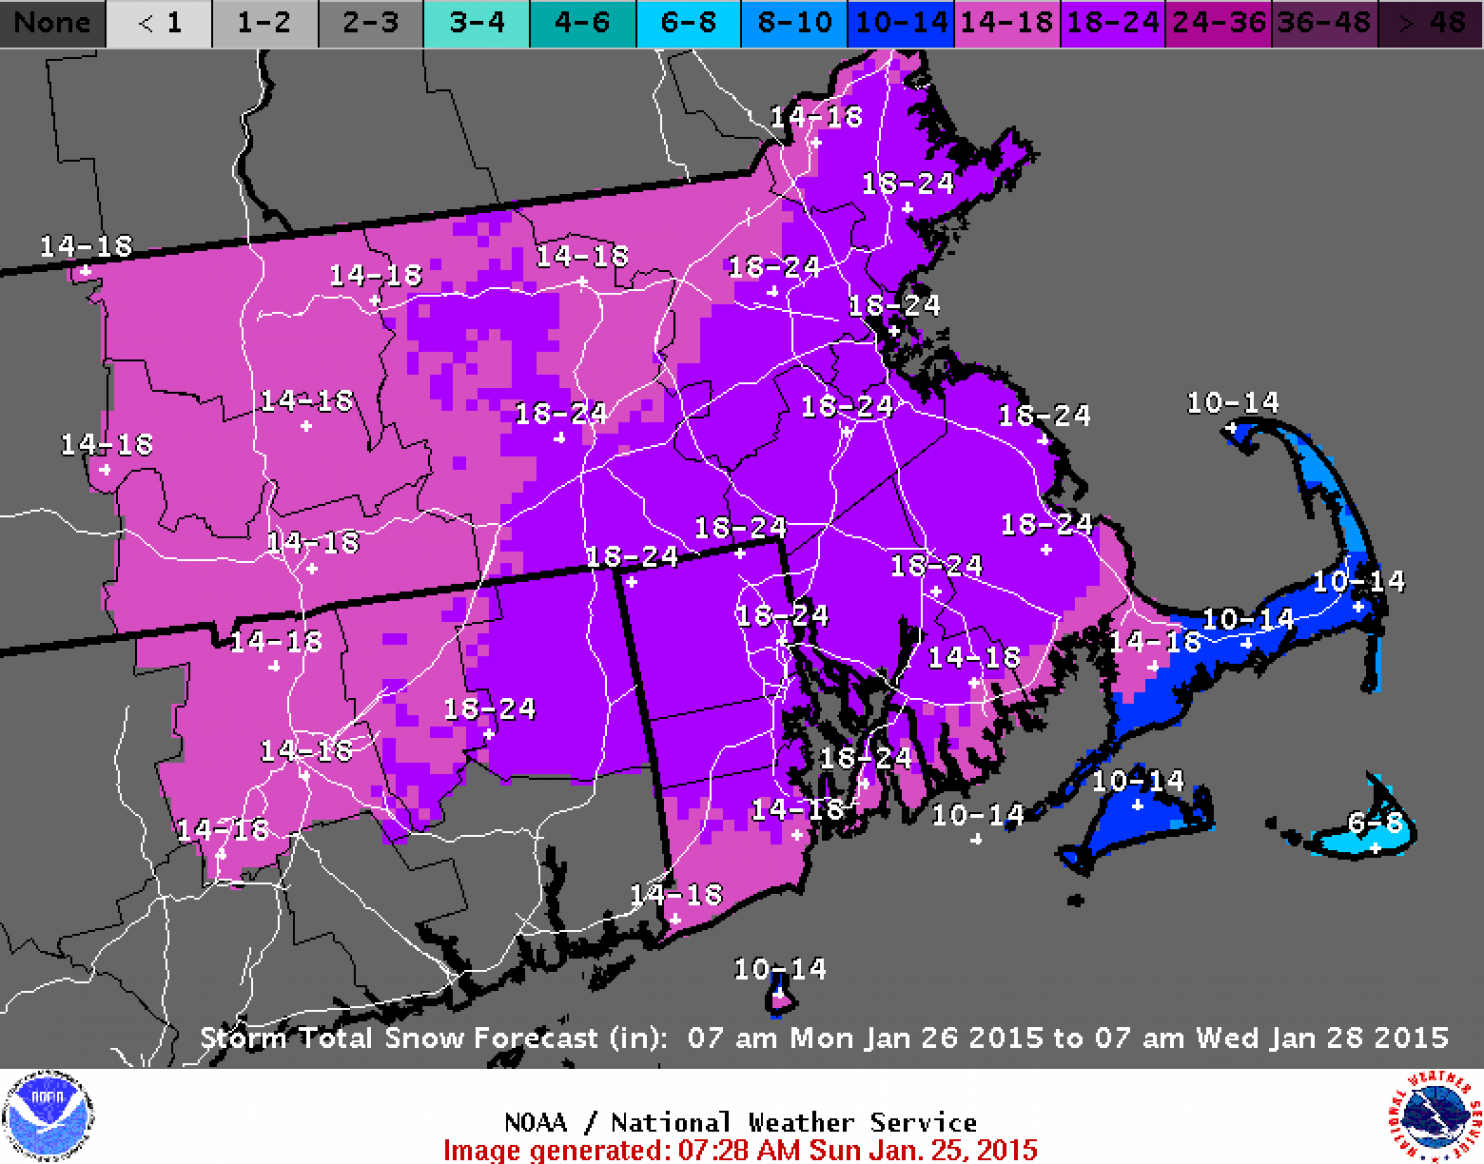
\includegraphics[width=3.5in]{../Figures/weather-forecast.png}
\end{frame}

\begin{frame}[t]{The Regression Learning Problem}
\begin{block}{Definition: Regression Learning Problem}
Given a data set of example pairs $\mathcal{D}=\{(\mbf{x}_i,y_i),i=1:N\}$ where $\mbf{x}_i\in\mathbb{R}^D$ is a feature vector and $y_i\in \mathbb{R}$ is the output, learn a function $f:\mathbb{R}^D\rightarrow \mathbb{R}$ that accurately predicts $y$ for any feature vector $\mbf{x}$.
\end{block}
\end{frame}

\begin{frame}[t]{Example: Linear Regression Learning}
\center
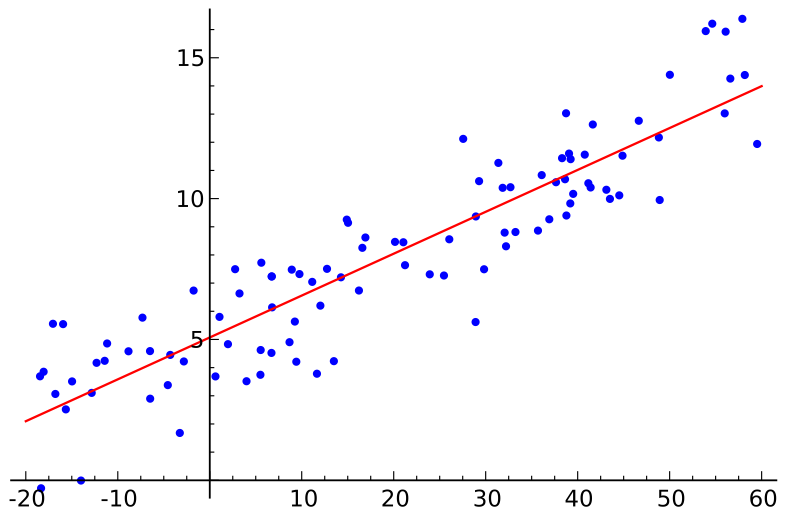
\includegraphics[width=3.5in]{../Figures/regression-learning-example.png}
\end{frame}

\begin{frame}[t]{Example: Non-Linear Regression Learning}
\center
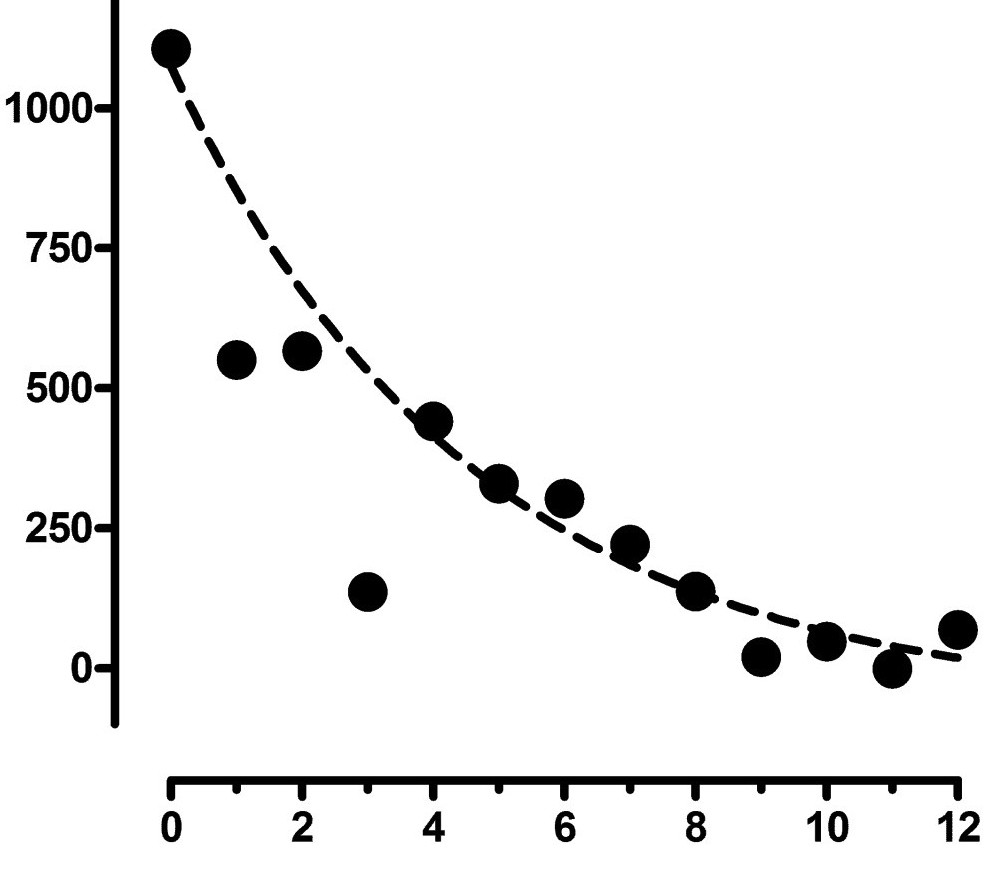
\includegraphics[width=3in]{../Figures/nonlinear-regression.jpg}
\end{frame}


\begin{frame}[t]{Error Measures: MSE}
\begin{block}{Definition: Mean Squared Error}
Given a data set of example pairs $\mathcal{D}=\{(\mbf{x}_i,y_i),i=1:N\}$ and a function $f:\mathbb{R}^D\rightarrow \mathcal{Y}$, the mean squared error of $f$ on $\mathcal{D}$ is:
$$MSE(f,\mathcal{D}) = \frac{1}{N}\sum_{i=1}^N(y_i - f(\mbf{x}_i))^2$$
\end{block}
\pause

Related measures include: \\
Sum of Squared Errors: $SSE(f,\mathcal{D})=N\cdot MSE(f,\mathcal{D})$\\
Risidual Sum of Squares: $RSS(f,\mathcal{D})=N\cdot MSE(f,\mathcal{D})$\\
Root Mean Squared Error: $RMSE(f,\mathcal{D})=\sqrt{MSE(f,\mathcal{D})}$


\end{frame}

\begin{frame}[t]{Error Measures: MAE}

\begin{block}{Definition: Mean Absolute Error}
Given a data set of example pairs $\mathcal{D}=\{(\mbf{x}_i,y_i),i=1:N\}$ and a function $f:\mathbb{R}^D\rightarrow \mathcal{Y}$, the mean absolute error of $f$ on $\mathcal{D}$ is:
$$MAE(f,\mathcal{D}) = \frac{1}{N}\sum_{i=1}^N|y_i - f(\mbf{x}_i)|$$
\end{block}

\end{frame}

\section{Linear regression}
\subsection{foo}

\begin{frame}[t]{Linear Regression}

Linear regression is a parametric regression method that assumes the relationship between $y$ and $\mbf{x}$ is a linear function with parameters $\mbf{w}=[w_1,...,w_D]^T$ and $b$.

\pause
\begin{block}{Linear Regression Function}
$$f_{Lin}(\mbf{x}) = \left(\sum_{d=1}^D w_d x_d\right) + b = \mbf{x}\mbf{w}+b$$
\end{block}

\pause \textbf{Question:} How can we learn the parameter values $\mbf{w}$ and $b$? 
\end{frame}

\begin{frame}[t]{Ordinary Least Squares Linear Regression}

Ordinary least squares selects the linear regression parameters to minimize the 
mean squared error (MSE) on the training data set:

\pause 
$$\mbf{w}^*,b^* = \argmin_{\mbf{w},b} \frac{1}{N}\sum_{i=1}^N(y_i - \mbf{x}_i\mbf{w}+b)^2$$

\end{frame}

\begin{frame}[t]{Solving OLS For One Feature}

$$\argmin_{w,b} \frac{1}{N}\sum_{i=1}^N(y_i - wx_i-b)^2$$
\pause
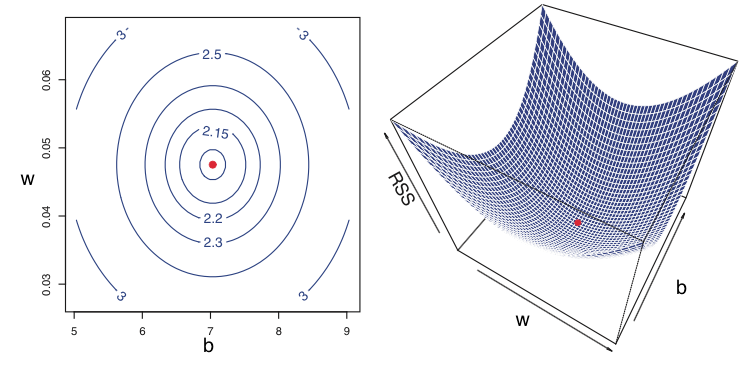
\includegraphics[width=4in]{../Figures/ols_objective.png}

\end{frame}

\begin{frame}[t]{Solving OLS For One Feature}

$$\argmin_{w,b} \frac{1}{N}\sum_{i=1}^N(y_i - wx_i-b)^2$$
\pause
\begin{align*}
\deriv{}{w}\frac{1}{N}\sum_{i=1}^N(y_i - wx_i-b)^2&=0\\
\deriv{}{b}\frac{1}{N}\sum_{i=1}^N(y_i - wx_i-b)^2&=0\\
\end{align*}

\end{frame}


\begin{frame}[t]{Solving OLS For One Feature}

\begin{align*}
2\frac{1}{N}\sum_{i=1}^N(y_i - wx_i-b)x_i&=0\\
2\frac{1}{N}\sum_{i=1}^N(y_i - wx_i-b)&=0
\end{align*}

\pause%
\begin{align*}
w\left(\sum_{i=1}^Nx_i^2\right) + b\left(\sum_{i=1}^Nx_i\right) &=\sum_{i=1}^N(y_ix_i)\\
w\left(\sum_{i=1}^Nx_i\right)+b(N)&= \sum_{i=1}^N(y_i) 
\end{align*}

\end{frame}

\begin{frame}[t]{Solving OLS For One Feature}

\begin{align*}
\begin{bmatrix}
\sum_{i=1}^Nx_i^2 & \sum_{i=1}^Nx_i \\
\sum_{i=1}^Nx_i   & N\\
\end{bmatrix}
\begin{bmatrix}
w\\
b
\end{bmatrix}
=
\begin{bmatrix}
\sum_{i=1}^Ny_ix_i \\
\sum_{i=1}^Ny_i 
\end{bmatrix}
\end{align*}
%
\pause
\begin{align*}
\begin{bmatrix}
w\\
b
\end{bmatrix}
=
\begin{bmatrix}
\sum_{i=1}^Nx_i^2 & \sum_{i=1}^Nx_i \\
\sum_{i=1}^Nx_i   & N\\
\end{bmatrix}^{-1}
\begin{bmatrix}
\sum_{i=1}^Ny_ix_i \\
\sum_{i=1}^Ny_i 
\end{bmatrix}
\end{align*}


\end{frame}

\begin{frame}[t]{General OLS Solution} 
Assume that $\mbf{X}$ is a data matrix with one data case $\mbf{x}_i\in \mathbb{R}^D$ per row, and $\mbf{Y}$ is 
a column vector containing the corresponding outputs. The general OLS solution is: 
\pause
\begin{align*}
\mbf{w}^* &= \argmin_{\mbf{w}} \frac{1}{N}\sum_{i=1}^N(y_i - \mbf{x}_i\mbf{w})^2\\
          &= \argmin_{\mbf{w}} \frac{1}{N}(\mbf{Y} - \mbf{X}\mbf{w})^T(\mbf{Y} - \mbf{X}\mbf{w})\\
0          &= \deriv{}{\mbf{w}} \frac{1}{N}(\mbf{Y} - \mbf{X}\mbf{w})^T(\mbf{Y} - \mbf{X}\mbf{w})\\
0&=\mbf{X}^T(\mbf{Y} - \mbf{X}\mbf{w}) \\
\mbf{X}^T\mbf{X}\mbf{w} &= \mbf{X}^T\mbf{Y}\\
\mbf{w}^* & = (\mbf{X}^T\mbf{X})^{-1}\mbf{X}^T\mbf{Y}
\end{align*}
\end{frame}

\begin{frame}[t]{Connection to Probabilistic Models} 
This same solution can be derived as the maximum conditional 
likelihood estimate for the parameters of a conditional 
Normal model. $\sigma^2$ is the noise variance.

\pause
\begin{align*}
P(y|\mbf{x}) = \mathcal{N}(y;\mbf{x}\mbf{w}, \sigma^2)
             = \frac{1}{\sqrt{2\pi\sigma^2}}\exp\left(-\frac{1}{2\sigma^2}(y-\mbf{x}\mbf{w})^2\right)
\end{align*}

\pause This view shows that OLS assumes the residuals are Normally distributed.
This assumption is violated in many real world processes that have significant
outliers or heavy-tailed noise.


\end{frame}

\begin{frame}[t]{Strengths and Limitations of OLS} 

\begin{itemize}
\item Need at least $D$ data cases to learn a model with a $D$
dimensional feature vector. \pause Otherwise inverse of
$\mbf{X}^T\mbf{X}$ is not defined.

\pause\item Very sensitive to noise and outliers due to MSE objective 
function/Normally distributed residuals assumption.

\pause\item Sensitive to co-linear features ($x_i \approx ax_j +b$). \pause Otherwise inverse of
$\mbf{X}^T\mbf{X}$ is not numerically stable.

\pause\item High bias (assumes linear relationships between the features and target).

\pause\item Computation is cubic in data dimension $D$.

\pause\item Variance is generally low unless there are outliers.


\end{itemize}

\end{frame}



\section{Regularization}
\subsection{foo}

\begin{frame}[t]{Regularized Linear Regression} 
Just as in classification, regression models require capacity control to avoid overfitting 
and numerical stability problems in high dimensions. This is accomplished by 
regularizing the weight parameters during learning.

\pause
\begin{align*}
\mbf{w}^* &= \argmin_{\mbf{w}} \frac{1}{N}\sum_{i=1}^N(y_i - \mbf{x}_i\mbf{w})^2 + \lambda ||\mbf{w}||\\
          &= \argmin_{\mbf{w}} \frac{1}{N}\sum_{i=1}^N(y_i - \mbf{x}_i\mbf{w})^2 
           \mbox{ ... st } ||\mbf{w}|| \leq c
\end{align*}
\end{frame}

\begin{frame}[t]{Ridge Regression} 
Ridge regression is the name given to regularized least squares when the weights are penalized using the square
of the $\ell_2$ norm $||\mbf{w}||_2^2 = \mbf{w}^T\mbf{w} = \sum_{d=1}^D w_d^2 $:

\pause
\begin{align*}
\mbf{w}^* &= \argmin_{\mbf{w}} \frac{1}{N}\sum_{i=1}^N(y_i - \mbf{x}_i\mbf{w})^2 + \lambda ||\mbf{w}||_2^2\\
          &= \argmin_{\mbf{w}} \frac{1}{N}\sum_{i=1}^N(y_i - \mbf{x}_i\mbf{w})^2 
          \mbox{ ... st } ||\mbf{w}||_2^2 \leq c
\end{align*}

\pause
In this case, it is easy to show that the optimal regularized weights are:

$$\mbf{w}^*  = (\mbf{X}^T\mbf{X}+\lambda I)^{-1}\mbf{X}^T\mbf{Y}$$

\end{frame}

\begin{frame}[t]{The Lasso} 
The Lasso is the name given to regularized least squares when the weights are penalized using the the $\ell_1$ norm $||\mbf{w}||_1 = \sum_{d=1}^D |w_d|$:

\pause
\begin{align*}
\mbf{w}^* &= \argmin_{\mbf{w}} \frac{1}{N}\sum_{i=1}^N(y_i - \mbf{x}_i\mbf{w})^2 + \lambda ||\mbf{w}||_1\\
          &= \argmin_{\mbf{w}} \frac{1}{N}\sum_{i=1}^N(y_i - \mbf{x}_i\mbf{w})^2 
          \mbox{ ... st } ||\mbf{w}||_1 \leq c
\end{align*}

\pause
The Lasso problem is a quadratic programming problem. However, it can be solved efficiently for all values of
$\lambda$ using an algorithm called \textit{least angle regression} (LARS). The advantage of the Lasso is that
it simultaneously performs regularization and feature selection.
\end{frame}

\begin{frame}[t]{Lasso vs Ridge} 

\center
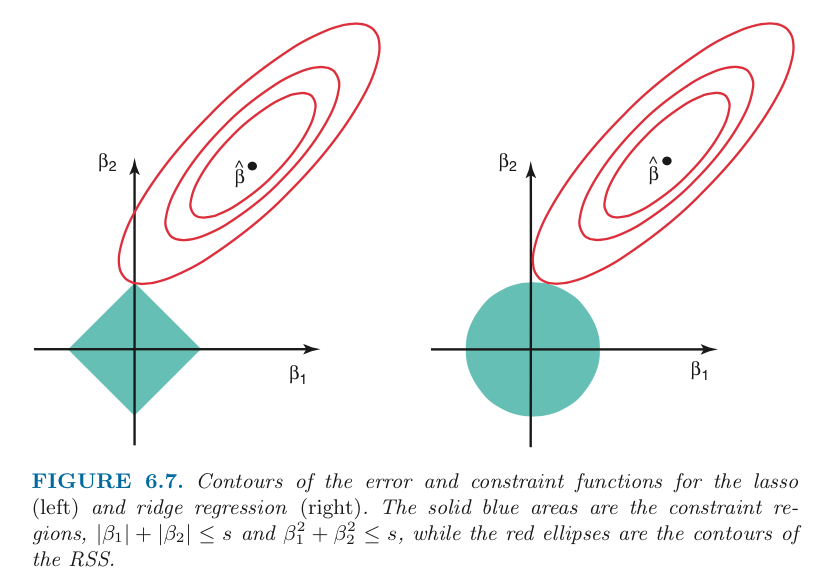
\includegraphics[width=4in]{../Figures/ridge_vs_lasso.png}

\end{frame}

\begin{frame}[t]{Strengths and Limitations of Ridge and Lasso} 

\begin{itemize}
\item Solves the problem of needing at least $D$ data cases to learn a model with a $D$
dimensional feature vector.

\pause\item Solves the problem of co-linear features ($x_i \approx ax_j +b$).

\pause\item MSE objective function still sensitive to noise and outliers, but regularization
can reduce the possibility of very large weights overfitting to outliers.

\pause\item Does not solve bias problem

\pause\item Computation for ridge is still cubic in data dimension $D$, but now need to
determine regularization parameters. Computation for LARS is similar.


\end{itemize}

\end{frame}

\section{Basis Expansion}
\subsection{foo}

\begin{frame}[t]{Basis Expansion} 
Just as with linear classification models, linear regression models can be extended to
capture non-linear relationships using basis function expansions. The polynomial basis is
often used for this purpose, although it is not sensible for forecasting.

\pause
\center
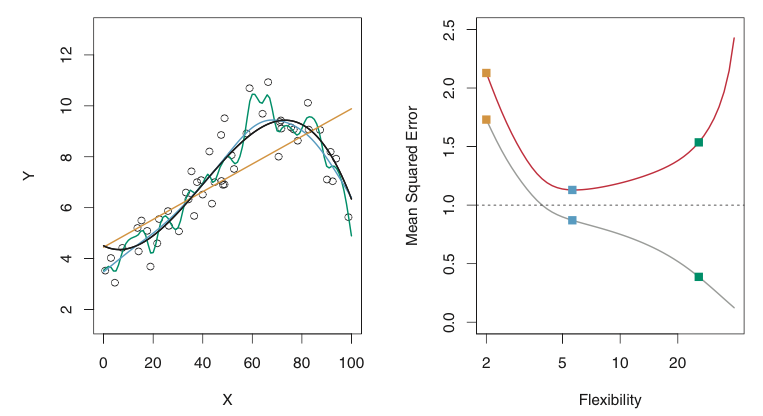
\includegraphics[width=4in]{../Figures/polynomial_regression.png}

\end{frame}


\begin{frame}[t]{Strengths and Limitations of Basis Expansion} 

\begin{itemize}
\item Does solve the bias problem.

\pause\item MSE objective function still sensitive to noise and outliers. Basis expansions
can easily overfit so need to control capacity.

\pause\item Computation is cubic in the dimensionality of the basis function
expansion. Can be costly.

\end{itemize}

\end{frame}




\end{document}
